\documentclass[10.5pt,a4paper]{article}
\usepackage[a4paper,margin=2.1cm,top=2.0cm,bottom=2.2cm]{geometry}
\usepackage{fontspec}
\setmainfont{IBMPlexSans}[
  Path = ../fonts/,
  Extension = .ttf,
  UprightFont = *-Regular,
  ItalicFont = *-Italic,
  BoldFont = *-SemiBold,
  BoldItalicFont = *-Italic]
\setmonofont{IBMPlexMono}[
  Extension = .otf,
  UprightFont = *-Regular,
  ItalicFont = *-Italic,
  BoldFont = *-SemiBold,
  Scale = MatchLowercase]
\usepackage{unicode-math}
\setmathfont{IBMPlexMath-Regular.otf}
\usepackage{xeCJK}
\setCJKmainfont{Microsoft YaHei}[BoldFont={Microsoft YaHei Bold},AutoFakeSlant=0.18]
\setCJKsansfont{Microsoft YaHei}[BoldFont={Microsoft YaHei Bold}]
\setCJKmonofont{Microsoft YaHei}
\xeCJKsetup{CJKecglue={\hskip 0.15em plus 0.05em minus 0.05em}}
\renewcommand{\figurename}{图}
\renewcommand{\tablename}{表}
\renewcommand{\refname}{参考文献}
\usepackage{graphicx}
\graphicspath{{../figures/}{../slides/assets/}}
\usepackage{booktabs}
\usepackage{tabularx}
\usepackage{array}
\usepackage{multirow}
\usepackage[font=small,skip=5pt,justification=justified,singlelinecheck=false]{caption}
\usepackage{xcolor}
\definecolor{bnmuted}{HTML}{6B7280}
\definecolor{nusblue}{HTML}{003D7C}
\definecolor{nusorange}{HTML}{EF7C00}
\usepackage[colorlinks=true,linkcolor=black,urlcolor=black,citecolor=black]{hyperref}
\usepackage{enumitem}
\setlist{nosep,leftmargin=1.2em}
\usepackage{float}
\usepackage{flafter}
\setcounter{topnumber}{3}
\setcounter{totalnumber}{4}
\renewcommand{\topfraction}{0.9}
\renewcommand{\textfraction}{0.08}
\renewcommand{\floatpagefraction}{0.75}
\setlength{\textfloatsep}{12pt plus 3pt minus 2pt}
\setlength{\floatsep}{10pt plus 2pt minus 2pt}
\setlength{\intextsep}{10pt plus 2pt minus 2pt}
\makeatletter
\setlength{\@fptop}{0pt}
\setlength{\@fpsep}{14pt plus 2pt}
\setlength{\@fpbot}{0pt plus 1fil}
\makeatother
\usepackage{titlesec}
\setcounter{secnumdepth}{2}
\titleformat{\section}{\large\bfseries\color{nusblue}}{\thesection}{0.6em}{}
\titleformat{\subsection}{\normalsize\bfseries\color{nusblue}}{\thesubsection}{0.6em}{}
\titlespacing*{\section}{0pt}{14pt}{6pt}
\titlespacing*{\subsection}{0pt}{10pt}{4pt}
\usepackage{indentfirst}
\setlength{\parindent}{1.5em}
\setlength{\parskip}{0pt plus 1pt}
\linespread{1.25}
\usepackage{fancyhdr}
\pagestyle{fancy}
\fancyhf{}
\renewcommand{\headrulewidth}{0pt}
\fancyfoot[L]{\footnotesize\color{bnmuted}BN5211 期末项目 课题 1：基于运动学与视频的手术技能评估（中文版）}
\fancyfoot[R]{\footnotesize\color{bnmuted}\thepage}
\usepackage[numbers,sort&compress]{natbib}
\setlength{\bibsep}{1pt}
\renewcommand{\bibfont}{\small}
\renewcommand{\bibsection}{\section{参考文献}}

%% Team information (shared by the English and Chinese reports and slides).
%% Member names and student IDs are kept out of the public repository.
\newcommand{\GroupName}{Group 17}
\newcommand{\TeamMembers}{National University of Singapore}
\newcommand{\ReportDate}{November 2026}

%% generated by code/make_tables.py from results/results.json -- do not edit
\newcommand{\FMZero}{0.218}
\newcommand{\AccMZero}{0.487}
\newcommand{\AccPctMZero}{48.7}
\newcommand{\LoMZero}{0.074}
\newcommand{\HiMZero}{0.310}
\newcommand{\PMZero}{1.000}
\newcommand{\FNMZero}{0.66}
\newcommand{\FIMZero}{0.00}
\newcommand{\FEMZero}{0.00}
\newcommand{\FoldAccMZero}{0.50}
\newcommand{\FoldSdMZero}{0.53}
\newcommand{\UBMZero}{5/5}
\newcommand{\UCMZero}{0/5}
\newcommand{\UDMZero}{0/5}
\newcommand{\UEMZero}{0/5}
\newcommand{\UFMZero}{0/5}
\newcommand{\UGMZero}{5/5}
\newcommand{\UHMZero}{4/4}
\newcommand{\UIMZero}{5/5}
\newcommand{\FMOne}{0.515}
\newcommand{\AccMOne}{0.615}
\newcommand{\AccPctMOne}{61.5}
\newcommand{\LoMOne}{0.272}
\newcommand{\HiMOne}{0.618}
\newcommand{\PMOne}{0.033}
\newcommand{\FNMOne}{0.75}
\newcommand{\FIMOne}{0.64}
\newcommand{\FEMOne}{0.15}
\newcommand{\FoldAccMOne}{0.62}
\newcommand{\FoldSdMOne}{0.34}
\newcommand{\UBMOne}{4/5}
\newcommand{\UCMOne}{4/5}
\newcommand{\UDMOne}{1/5}
\newcommand{\UEMOne}{0/5}
\newcommand{\UFMOne}{4/5}
\newcommand{\UGMOne}{5/5}
\newcommand{\UHMOne}{3/4}
\newcommand{\UIMOne}{3/5}
\newcommand{\FMTwoA}{0.345}
\newcommand{\AccMTwoA}{0.436}
\newcommand{\AccPctMTwoA}{43.6}
\newcommand{\LoMTwoA}{0.125}
\newcommand{\HiMTwoA}{0.496}
\newcommand{\PMTwoA}{0.455}
\newcommand{\FNMTwoA}{0.72}
\newcommand{\FIMTwoA}{0.00}
\newcommand{\FEMTwoA}{0.32}
\newcommand{\FoldAccMTwoA}{0.45}
\newcommand{\FoldSdMTwoA}{0.50}
\newcommand{\UBMTwoA}{0/5}
\newcommand{\UCMTwoA}{0/5}
\newcommand{\UDMTwoA}{0/5}
\newcommand{\UEMTwoA}{3/5}
\newcommand{\UFMTwoA}{0/5}
\newcommand{\UGMTwoA}{5/5}
\newcommand{\UHMTwoA}{4/4}
\newcommand{\UIMTwoA}{5/5}
\newcommand{\FMTwoB}{0.371}
\newcommand{\AccMTwoB}{0.487}
\newcommand{\AccPctMTwoB}{48.7}
\newcommand{\LoMTwoB}{0.222}
\newcommand{\HiMTwoB}{0.467}
\newcommand{\PMTwoB}{0.348}
\newcommand{\FNMTwoB}{0.75}
\newcommand{\FIMTwoB}{0.36}
\newcommand{\FEMTwoB}{0.00}
\newcommand{\FoldAccMTwoB}{0.49}
\newcommand{\FoldSdMTwoB}{0.38}
\newcommand{\UBMTwoB}{4/5}
\newcommand{\UCMTwoB}{3/5}
\newcommand{\UDMTwoB}{0/5}
\newcommand{\UEMTwoB}{0/5}
\newcommand{\UFMTwoB}{1/5}
\newcommand{\UGMTwoB}{5/5}
\newcommand{\UHMTwoB}{3/4}
\newcommand{\UIMTwoB}{3/5}
\newcommand{\FMTwoC}{0.420}
\newcommand{\AccMTwoC}{0.513}
\newcommand{\AccPctMTwoC}{51.3}
\newcommand{\LoMTwoC}{0.178}
\newcommand{\HiMTwoC}{0.576}
\newcommand{\PMTwoC}{0.240}
\newcommand{\FNMTwoC}{0.67}
\newcommand{\FIMTwoC}{0.59}
\newcommand{\FEMTwoC}{0.00}
\newcommand{\FoldAccMTwoC}{0.50}
\newcommand{\FoldSdMTwoC}{0.47}
\newcommand{\UBMTwoC}{5/5}
\newcommand{\UCMTwoC}{5/5}
\newcommand{\UDMTwoC}{0/5}
\newcommand{\UEMTwoC}{0/5}
\newcommand{\UFMTwoC}{3/5}
\newcommand{\UGMTwoC}{5/5}
\newcommand{\UHMTwoC}{0/4}
\newcommand{\UIMTwoC}{2/5}
\newcommand{\FMThree}{0.443}
\newcommand{\AccMThree}{0.538}
\newcommand{\AccPctMThree}{53.8}
\newcommand{\LoMThree}{0.247}
\newcommand{\HiMThree}{0.568}
\newcommand{\PMThree}{0.188}
\newcommand{\FNMThree}{0.75}
\newcommand{\FIMThree}{0.45}
\newcommand{\FEMThree}{0.12}
\newcommand{\FoldAccMThree}{0.54}
\newcommand{\FoldSdMThree}{0.36}
\newcommand{\UBMThree}{4/5}
\newcommand{\UCMThree}{4/5}
\newcommand{\UDMThree}{1/5}
\newcommand{\UEMThree}{0/5}
\newcommand{\UFMThree}{1/5}
\newcommand{\UGMThree}{5/5}
\newcommand{\UHMThree}{3/4}
\newcommand{\UIMThree}{3/5}
\newcommand{\FMThreeB}{0.450}
\newcommand{\AccMThreeB}{0.538}
\newcommand{\AccPctMThreeB}{53.8}
\newcommand{\LoMThreeB}{0.253}
\newcommand{\HiMThreeB}{0.567}
\newcommand{\PMThreeB}{0.133}
\newcommand{\FNMThreeB}{0.72}
\newcommand{\FIMThreeB}{0.50}
\newcommand{\FEMThreeB}{0.13}
\newcommand{\FoldAccMThreeB}{0.54}
\newcommand{\FoldSdMThreeB}{0.33}
\newcommand{\UBMThreeB}{3/5}
\newcommand{\UCMThreeB}{2/5}
\newcommand{\UDMThreeB}{1/5}
\newcommand{\UEMThreeB}{0/5}
\newcommand{\UFMThreeB}{4/5}
\newcommand{\UGMThreeB}{5/5}
\newcommand{\UHMThreeB}{3/4}
\newcommand{\UIMThreeB}{3/5}
\newcommand{\FMThreeC}{0.481}
\newcommand{\AccMThreeC}{0.615}
\newcommand{\AccPctMThreeC}{61.5}
\newcommand{\LoMThreeC}{0.236}
\newcommand{\HiMThreeC}{0.596}
\newcommand{\PMThreeC}{0.062}
\newcommand{\FNMThreeC}{0.75}
\newcommand{\FIMThreeC}{0.69}
\newcommand{\FEMThreeC}{0.00}
\newcommand{\FoldAccMThreeC}{0.62}
\newcommand{\FoldSdMThreeC}{0.40}
\newcommand{\UBMThreeC}{4/5}
\newcommand{\UCMThreeC}{4/5}
\newcommand{\UDMThreeC}{0/5}
\newcommand{\UEMThreeC}{0/5}
\newcommand{\UFMThreeC}{5/5}
\newcommand{\UGMThreeC}{5/5}
\newcommand{\UHMThreeC}{3/4}
\newcommand{\UIMThreeC}{3/5}
\newcommand{\FMThreeD}{0.461}
\newcommand{\AccMThreeD}{0.615}
\newcommand{\AccPctMThreeD}{61.5}
\newcommand{\LoMThreeD}{0.242}
\newcommand{\HiMThreeD}{0.564}
\newcommand{\PMThreeD}{0.036}
\newcommand{\FNMThreeD}{0.74}
\newcommand{\FIMThreeD}{0.64}
\newcommand{\FEMThreeD}{0.00}
\newcommand{\FoldAccMThreeD}{0.62}
\newcommand{\FoldSdMThreeD}{0.41}
\newcommand{\UBMThreeD}{4/5}
\newcommand{\UCMThreeD}{4/5}
\newcommand{\UDMThreeD}{0/5}
\newcommand{\UEMThreeD}{0/5}
\newcommand{\UFMThreeD}{4/5}
\newcommand{\UGMThreeD}{5/5}
\newcommand{\UHMThreeD}{4/4}
\newcommand{\UIMThreeD}{3/5}
\newcommand{\FMFour}{0.520}
\newcommand{\AccMFour}{0.615}
\newcommand{\AccPctMFour}{61.5}
\newcommand{\LoMFour}{0.273}
\newcommand{\HiMFour}{0.619}
\newcommand{\PMFour}{0.074}
\newcommand{\FNMFour}{0.75}
\newcommand{\FIMFour}{0.67}
\newcommand{\FEMFour}{0.14}
\newcommand{\FoldAccMFour}{0.61}
\newcommand{\FoldSdMFour}{0.35}
\newcommand{\UBMFour}{4/5}
\newcommand{\UCMFour}{4/5}
\newcommand{\UDMFour}{1/5}
\newcommand{\UEMFour}{0/5}
\newcommand{\UFMFour}{4/5}
\newcommand{\UGMFour}{5/5}
\newcommand{\UHMFour}{2/4}
\newcommand{\UIMFour}{4/5}
\newcommand{\FMFive}{0.440}
\newcommand{\AccMFive}{0.538}
\newcommand{\AccPctMFive}{53.8}
\newcommand{\LoMFive}{0.259}
\newcommand{\HiMFive}{0.526}
\newcommand{\PMFive}{0.157}
\newcommand{\FNMFive}{0.73}
\newcommand{\FIMFive}{0.45}
\newcommand{\FEMFive}{0.13}
\newcommand{\FoldAccMFive}{0.54}
\newcommand{\FoldSdMFive}{0.33}
\newcommand{\UBMFive}{4/5}
\newcommand{\UCMFive}{3/5}
\newcommand{\UDMFive}{1/5}
\newcommand{\UEMFive}{0/5}
\newcommand{\UFMFive}{2/5}
\newcommand{\UGMFive}{5/5}
\newcommand{\UHMFive}{3/4}
\newcommand{\UIMFive}{3/5}
\newcommand{\FCOne}{0.375}
\newcommand{\AccCOne}{0.487}
\newcommand{\AccPctCOne}{48.7}
\newcommand{\LoCOne}{0.275}
\newcommand{\HiCOne}{0.482}
\newcommand{\PCOne}{0.367}
\newcommand{\FNCOne}{0.82}
\newcommand{\FICOne}{0.20}
\newcommand{\FECOne}{0.11}
\newcommand{\FoldAccCOne}{0.50}
\newcommand{\FoldSdCOne}{0.41}
\newcommand{\UBCOne}{4/5}
\newcommand{\UCCOne}{2/5}
\newcommand{\UDCOne}{0/5}
\newcommand{\UECOne}{1/5}
\newcommand{\UFCOne}{0/5}
\newcommand{\UGCOne}{3/5}
\newcommand{\UHCOne}{4/4}
\newcommand{\UICOne}{5/5}
\newcommand{\FCTwo}{0.342}
\newcommand{\AccCTwo}{0.385}
\newcommand{\AccPctCTwo}{38.5}
\newcommand{\LoCTwo}{0.167}
\newcommand{\HiCTwo}{0.475}
\newcommand{\PCTwo}{0.445}
\newcommand{\FNCTwo}{0.47}
\newcommand{\FICTwo}{0.43}
\newcommand{\FECTwo}{0.12}
\newcommand{\FoldAccCTwo}{0.38}
\newcommand{\FoldSdCTwo}{0.31}
\newcommand{\UBCTwo}{3/5}
\newcommand{\UCCTwo}{4/5}
\newcommand{\UDCTwo}{1/5}
\newcommand{\UECTwo}{0/5}
\newcommand{\UFCTwo}{1/5}
\newcommand{\UGCTwo}{4/5}
\newcommand{\UHCTwo}{1/4}
\newcommand{\UICTwo}{1/5}
\newcommand{\FCTwoT}{0.344}
\newcommand{\AccCTwoT}{0.385}
\newcommand{\AccPctCTwoT}{38.5}
\newcommand{\LoCTwoT}{0.132}
\newcommand{\HiCTwoT}{0.509}
\newcommand{\PCTwoT}{0.371}
\newcommand{\FNCTwoT}{0.38}
\newcommand{\FICTwoT}{0.53}
\newcommand{\FECTwoT}{0.12}
\newcommand{\FoldAccCTwoT}{0.38}
\newcommand{\FoldSdCTwoT}{0.37}
\newcommand{\UBCTwoT}{1/5}
\newcommand{\UCCTwoT}{5/5}
\newcommand{\UDCTwoT}{1/5}
\newcommand{\UECTwoT}{0/5}
\newcommand{\UFCTwoT}{3/5}
\newcommand{\UGCTwoT}{4/5}
\newcommand{\UHCTwoT}{1/4}
\newcommand{\UICTwoT}{0/5}
\newcommand{\DOneZero}{$+$0.296}
\newcommand{\DAbsOneZero}{0.296}
\newcommand{\DLoOneZero}{$+$0.015}
\newcommand{\DHiOneZero}{$+$0.443}
\newcommand{\DThreeOne}{$-$0.071}
\newcommand{\DAbsThreeOne}{0.071}
\newcommand{\DLoThreeOne}{$-$0.170}
\newcommand{\DHiThreeOne}{$+$0.010}
\newcommand{\DFourOne}{$+$0.005}
\newcommand{\DAbsFourOne}{0.005}
\newcommand{\DLoFourOne}{$-$0.043}
\newcommand{\DHiFourOne}{$+$0.051}
\newcommand{\DThreeBOne}{$-$0.064}
\newcommand{\DAbsThreeBOne}{0.064}
\newcommand{\DLoThreeBOne}{$-$0.133}
\newcommand{\DHiThreeBOne}{$+$0.000}
\newcommand{\DThreeCOne}{$-$0.034}
\newcommand{\DAbsThreeCOne}{0.034}
\newcommand{\DLoThreeCOne}{$-$0.111}
\newcommand{\DHiThreeCOne}{$+$0.050}
\newcommand{\DThreeDOne}{$-$0.053}
\newcommand{\DAbsThreeDOne}{0.053}
\newcommand{\DLoThreeDOne}{$-$0.128}
\newcommand{\DHiThreeDOne}{$+$0.019}
\newcommand{\DFiveFour}{$-$0.080}
\newcommand{\DAbsFiveFour}{0.080}
\newcommand{\DLoFiveFour}{$-$0.128}
\newcommand{\DHiFiveFour}{$+$0.014}
\newcommand{\DTwoBZero}{$+$0.153}
\newcommand{\DAbsTwoBZero}{0.153}
\newcommand{\DLoTwoBZero}{$-$0.020}
\newcommand{\DHiTwoBZero}{$+$0.259}
\newcommand{\IdKSimple}{0.92}
\newcommand{\IdKTexture}{0.89}
\newcommand{\IdDuration}{0.26}
\newcommand{\IdVAppear}{1.00}
\newcommand{\IdVDyn}{0.44}
\newcommand{\IdVFlow}{0.56}
\newcommand{\NTrials}{39}
\newcommand{\DurMin}{59}
\newcommand{\DurMax}{300}
\newcommand{\DurMedian}{105}
\newcommand{\DurN}{124}
\newcommand{\DurI}{84}
\newcommand{\DurE}{89}
\newcommand{\NFramesOneHz}{4406}
\newcommand{\NPairsTwoHz}{8794}
\newcommand{\PaceKSimple}{0.42}
\newcommand{\PaceVDyn}{0.54}
\newcommand{\PaceKTexture}{0.34}
\newcommand{\PaceVFlow}{0.35}
\newcommand{\PaceKTextureMax}{0.93}
\newcommand{\VerPython}{3.11.0}
\newcommand{\VerNumpy}{2.4.6}
\newcommand{\VerSklearn}{1.9.1}
\newcommand{\VerTorch}{2.11.0+cu128}
\newcommand{\VerTorchvision}{0.26.0+cu128}
\newcommand{\VerOpencv}{5.0.0}
\newcommand{\VerScipy}{1.17.1}
\newcommand{\VerPandas}{3.0.5}
\newcommand{\CaseGZeroOneDur}{300}
\newcommand{\CaseGZeroOnePPred}{0.98}
\newcommand{\CaseGZeroOnePTrue}{0.98}
\newcommand{\CaseCZeroFourDur}{83}
\newcommand{\CaseCZeroFourPPred}{0.91}
\newcommand{\CaseCZeroFourPTrue}{0.91}
\newcommand{\CaseEZeroOneDur}{120}
\newcommand{\CaseEZeroOnePPred}{0.69}
\newcommand{\CaseEZeroOnePTrue}{0.14}
\newcommand{\CaseDZeroFiveDur}{59}
\newcommand{\CaseDZeroFivePPred}{0.89}
\newcommand{\CaseDZeroFivePTrue}{0.04}
\newcommand{\CaseIZeroFiveDur}{126}
\newcommand{\CaseIZeroFivePPred}{0.93}
\newcommand{\CaseIZeroFivePTrue}{0.07}
\newcommand{\DurRangeD}{59--93}
\newcommand{\DurRangeE}{83--120}
\newcommand{\DurRangeCF}{68--109}

\newcommand{\pp}{\,pp}

\begin{document}
\noindent
\includegraphics[height=1.25cm]{NationalUniversityofSingapore.pdf}\par
\vspace{2pt}{\color{nusorange}\rule{\textwidth}{1.2pt}}\par\vspace{6pt}
\begin{center}
{\LARGE\bfseries\color{nusblue} 基于运动学与视频的手术技能评估}\\[3pt]
{\large 在留一用户评估下对 JIGSAWS 缝合任务的新手、中级与专家进行分类}\\[8pt]
{\normalsize BN5211 医疗机器人智能 期末项目（课题 1）\quad\textbar\quad \GroupName}\\[4pt]
{\small \TeamMembers}\\[2pt]
{\small\color{bnmuted} \ReportDate}
\end{center}
\vspace{2pt}
% the title and team block is item 1 of the required report structure, so Background is Section 2
\setcounter{section}{1}

\section{研究背景}

\subsection{临床与机器人学动机}

手术技术水平直接影响临床结局。一项针对减重外科医生的研究由同行对手术录像评分，评分最低四分位组的并发症、再次手术和再入院率明显高于评分最高四分位组\citep{birkmeyer2013skill}。目前技能评估主要依靠专家观察，并借助 OSATS 等结构化量表和整体评分\citep{martin1997osats}。这一过程耗时、昂贵且带有主观性，因此很难为受训者提供频繁反馈，也难以在资格认证中保持一致\citep{reiley2011review}。机器人辅助微创手术改变了这一局面，因为机器人本身就在记录外科医生的动作：da~Vinci 系统以固定频率记录每个机械臂的位姿、速度和夹钳角度，内窥镜则记录术野画面。客观技能评估因此可以基于本来就会采集的数据完成，这使它成为医疗机器人智能中的一个自然问题。这类模型只有在面对从未见过的外科医生时依然有效，才具有实际价值。被系统评估的受训者不会出现在训练集中，所以评估必须整体留出外科医生，而不是留出单个试次。

\subsection{相关工作}

JHU-ISI 手势与技能评估数据集（JIGSAWS）是该问题的标准公开基准\citep{gao2014jigsaws}。它包含八位外科医生在台式模型上完成缝合、打结和穿针任务时同步记录的运动学数据和立体视频，每个试次附有自报技能等级和改良 OSATS 评分。该数据集的基准协议区分留一超试次（LOSO，每位外科医生各留出一次重复）和留一用户（LOUO，留出某位外科医生的全部试次）两种划分\citep{ahmidi2017benchmarks}。基于运动学的方法大致分为三类。第一类用全局运动统计量概括一个试次，例如完成时间、路径长度、运动经济性和夹钳动作次数，这些指标与专家评分时关注的要素接近，计算代价也低\citep{reiley2011review, lefor2020motion, anh2020features}。第二类刻画运动信号的纹理。本课题的背景文献 \citet{zia2018rmis} 在每个运动学通道上计算近似熵\citep{pincus1991apen}等度量，用最近邻分类器在 LOUO 下报告了缝合任务 88.2\% 的准确率；同一团队也将这一思路用于视频和加速度计数据\citep{zia2018video}。第三类端到端学习特征，例如在原始运动学序列\citep{fawaz2018cnn, wang2018cnn}或视频片段\citep{funke2019video, liu2021unified}上训练卷积网络；近期的视频 Transformer 已能从临床录像中解码外科医生的动作和技能\citep{kiyasseh2023vit, lavanchy2021threestage}。许多最高的已发表结果采用 LOSO，此时每位测试外科医生也出现在训练集中，这种划分下接近 100\% 的准确率很常见\citep{fawaz2018cnn, funke2019video}。在 LOUO 下，任务变成仅凭七位训练外科医生去泛化到新的人，任何估计的不确定性都很大\citep{varoquaux2018cv}。因此两种划分得到的结果不可直接比较。类别分布带来了第二个难点。新手试次占缝合任务的将近一半，准确率因此会偏向倾向多数类的分类器；不平衡学习的文献建议采用类别平衡的训练方式，并使用对每个类别同等加权的指标，例如 macro-F1\citep{he2009imbalanced}。本文同时采用了这两项建议。

\subsection{方法选择的动机}

本课题规定了核心实验：用简单的试次级统计量构建仅运动学基线，加入来自采样帧或短片段的视频特征，评估一个简单的运动学与视频融合模型，并在 LOUO 下以 macro-F1 与多数类基线比较。我们的设计选择源于数据的两个性质。第一，JIGSAWS 缝合任务只有来自八位外科医生的 39 个可用试次，并且技能标签在同一外科医生内部恒定。因此学习“技能等级之间差异”的有效样本量更接近 8 而不是 39，中级和专家两类各只有两位外科医生。这一点更适合参数少、正则化强的低容量模型，而不是端到端深度网络；对视频我们使用冻结的预训练图像特征加线性分类器，不做任何微调。第二，由于标签属于外科医生，任何能识别外科医生身份的特征都能在训练集内预测标签，却并不反映技能。因此我们把捷径检测作为方法的一部分，在必做实验之外加入两项测量：一是各特征块在多大程度上编码了外科医生身份的探针，二是衡量决策中有多少可以由试次节奏解释的对照实验。作为针对性改进，我们检验背景文献的核心观点，即专业水平体现在动作的规律性上，而不仅仅体现在速度上，具体做法是在简单统计量之外加入运动纹理特征。所有模型、指标和比较都在计算第一个结果之前写入书面协议，因此最终报告哪个模型不会受到结果的影响。

\section{方法}

\subsection{数据与任务}

我们使用 JIGSAWS 官方发布版中的缝合（Suturing）任务。元数据文件列出了来自八位外科医生（用户 B 至 I）的 \NTrials{} 个试次。每位用户完成五个试次，只有用户 H 例外：其试次 H002 在官方发布版中没有标签和折划分条目，因此缺失。预测目标是自报技能等级：新手（N，机器人操作经验少于 10 小时）、中级（I，10 至 100 小时）或专家（E，超过 100 小时）。用户 B、G、H、I 为新手（19 个试次），C 和 F 为中级（10 个试次），D 和 E 为专家（10 个试次）。每个试次提供 30\,Hz 采样的 76 个运动学通道，即两个医生端主控臂和两个患者端器械各自的笛卡尔位置、旋转矩阵、线速度、角速度和夹钳角度，以及两路 640$\times$480 像素、每秒 30 帧的内窥镜视频。运动学特征只使用患者端器械，因为它们是真正作用于组织的工具，而在遥操作下主控臂信号与之高度重复；视频特征使用左侧相机视图（capture1）。试次时长在 \DurMin{} 至 \DurMax{}\,s 之间（中位数 \DurMedian{}\,s），新手平均更慢（图~\ref{fig:data}）。任何模型都不使用手势标注或 OSATS 评分。

\begin{figure}[htbp]
\centering
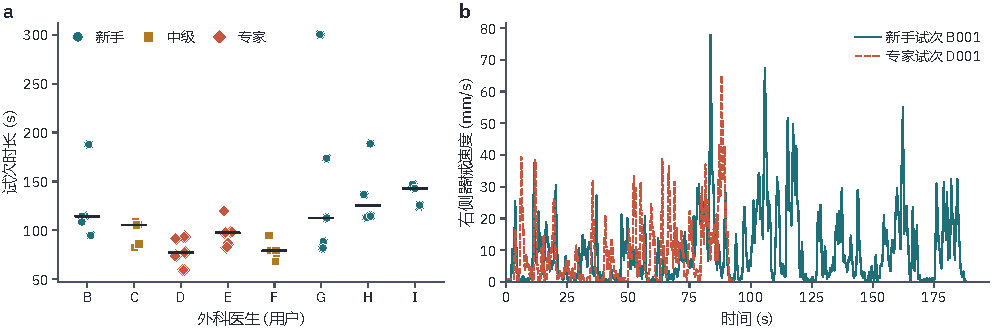
\includegraphics{fig2_data_zh.pdf}
\caption{(a) 各外科医生的试次时长，颜色表示技能等级，横线为中位数。(b) 一个新手试次（B001）和一个专家试次（D001）中右侧患者端器械的速度（0.5\,s 平滑）。专家用约一半的时间完成任务，峰值速度相近。}
\label{fig:data}
\end{figure}

\subsection{工作流程}

图~\ref{fig:pipeline} 概括了整个流程。每个试次被转换为若干定长特征向量，每个特征块对应一个向量。每个特征块由标准化后的 L2 正则逻辑回归分类，其正则化强度在训练外科医生内部选择。多模态模型要么在分类前拼接特征块（早期融合），要么对一个运动学分类器和一个视频分类器的类别概率取平均（后期融合）。所有模型都在 JIGSAWS 技能检测设置的八个官方 LOUO 折上评估。

\begin{figure}[htbp]
\centering
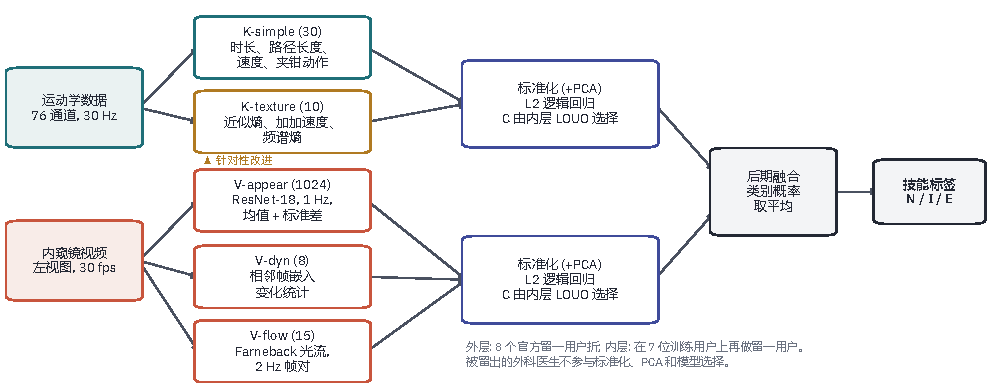
\includegraphics{fig1_pipeline_zh.pdf}
\caption{工作流程。每个试次提取运动学和视频特征块，由正则化逻辑回归分类；后期融合对一个运动学分类器和一个视频分类器的类别概率取平均。K-texture 特征块是本文的针对性改进。括号内数字为特征维数。所有拟合步骤（包括标准化、PCA 和正则化强度的选择）都只使用每一折的训练外科医生。}
\label{fig:pipeline}
\end{figure}

\subsection{运动学特征}

仅运动学基线（K-simple，30 维）实现了任务说明中点名的统计量。对每个患者端器械，我们计算：路径长度（相邻工具尖端位置间距离之和）；线速度的均值、标准差和第 90 百分位数；角速度的均值和标准差；静止比例，即线速度低于 5\,mm/s 的采样点所占比例；运动经济性，即路径长度除以工具尖端轨迹包围盒的对角线长度；以及五个夹钳统计量，即夹钳角度的均值、标准差、范围、总绝对变化量和开合次数（以 0.5\,s 滑动平均信号向上穿越其均值的次数计）。另有四个试次级特征：时长（秒）、两个器械速度之间的相关系数、两者同时静止的时间比例，以及两条路径长度之比的对数。这些都是描述效率和双手协调的常用指标\citep{reiley2011review, lefor2020motion}。

运动纹理特征块（K-texture，10 维）是本文的针对性改进，参照背景文献\citep{zia2018rmis}设计。对每个器械，我们计算线速度、角速度和夹钳角度的近似熵\citep{pincus1991apen}（均重采样到 10\,Hz，嵌入维数 $m = 2$，容差 $r$ 取信号标准差的 0.2 倍）；速度曲线的对数无量纲加加速度（log dimensionless jerk）\citep{hogan2009smoothness}；以及速度的归一化频谱熵。这些特征描述的是动作有多规律、多平滑，而不是多快或多长；按设想，即使两人用时相近，这一性质也应能区分动作流畅的专家和犹豫不决的新手。

\subsection{视频特征}

每个试次的视频只解码一遍。每 30 帧取一帧（1\,Hz，共 \NFramesOneHz{} 帧），缩放到 224$\times$224 像素后输入去掉分类层的 ImageNet 预训练 ResNet-18\citep{he2016resnet}，得到每帧 512 维嵌入。外观特征块（V-appear，1024 维）是这些嵌入在整个试次上的均值和标准差；由于 1024 维对 34 个训练试次而言维数过高，我们在每个训练折内拟合 4、8 或 16 个主成分的 PCA。场景动态特征块（V-dyn，8 维）概括画面变化的快慢：由相邻 1\,Hz 嵌入之间的余弦距离取均值、标准差、第 10/50/90 百分位数和变异系数，由欧氏距离取均值和标准差。某一录制场次中恒定的外观成分（例如光照或练习板的摆放）在差分中相互抵消，因此 V-dyn 携带的录制环境信息应少于 V-appear，同时仍能反映器械运动和组织变化。光流特征块（V-flow，15 维）在以 2\,Hz 采样、缩放到 320$\times$240 像素的相邻帧对（共 \NPairsTwoHz{} 对）上计算 Farneback 稠密光流\citep{farneback2003flow}。对每个帧对，我们计算光流幅值的均值、标准差和第 90 百分位数、运动速度超过每帧 0.5 像素的像素比例，以及按幅值加权的 8 方向光流方向熵；这五个序列再分别用试次内的均值、标准差和第 90 百分位数概括。

\subsection{分类器与融合}

所有特征块使用同一模型：标准化、可选的 PCA（仅 V-appear）、PCA 后再次标准化，以及带 L2 惩罚、类别平衡权重和 L-BFGS 求解器的多项逻辑回归\citep{pedregosa2011sklearn}。逆正则化强度 $C$ 从 $\{0.01, 0.03, 0.1, 0.3, 1, 3, 10\}$ 中选择，V-appear 的主成分数从 $\{4, 8, 16\}$ 中选择。后期融合以相等权重平均运动学分类器和一个视频分类器的类别概率；采用等权重是因为 34 个训练试次不足以可靠地估计融合权重。早期融合把 K-simple 与 V-dyn 拼接后拟合一个分类器。主多模态模型在看到任何结果之前就已确定，即 K-simple 与 V-dyn 的后期融合（M3）。选择 V-dyn 作为主视频特征块，一是出于上面所述的基本原理，二是因为本组此前在同样 39 个试次上的探索性分析发现嵌入变化统计量是最有希望的视频描述符。由于那次分析看过同一数据上的折外结果，这一选择并非完全不受选择偏差影响，因此我们报告全部三个视频特征块和全部四种融合变体。

\subsection{评估协议}

我们使用 \texttt{Suturing/unBalanced/SkillDetection/UserOut} 中的 JIGSAWS 官方折；代码检查每一折恰好留出一位外科医生，共八折，每折训练试次为 34 或 35 个。超参数由每个外层折内、在七位训练外科医生上进行的内层 LOUO 循环选择，以内层合并 macro-F1 最大为准，平局时取更强的正则化。当外层折留出的是中级或专家外科医生时，该类只剩一位外科医生，内层留出它的那一折就没有该类的训练样本；这样的内层折被跳过（每个受影响的外层折跳过一个）。因此被留出的外科医生从不影响标准化、PCA、特征残差化或模型选择。

主要指标是在 39 个合并的折外预测上一次性计算的 macro-F1。由于标签在同一外科医生内部恒定，每个 LOUO 测试折只含一个类别，另外两个缺失类别的逐折 macro-F1 没有定义，所以合并计算是该指标唯一良好定义的形式。我们同时报告准确率、各类别 F1、混淆矩阵和每位外科医生的准确率。只有八位外科医生时不确定性很大，因此我们用两种尊重试次分组结构的方法加以量化。用户级 bootstrap 对八位外科医生有放回地重采样 2000 次，给出 macro-F1 及模型间配对差值的百分位区间。精确置换检验在外科医生之间重新分配技能标签，同时保持每位外科医生的试次在一起；四位新手、两位中级、两位专家共有 $8!/(4!\,2!\,2!) = 420$ 种不同的分配方式，因此固定预测下 macro-F1 的零分布可以被精确枚举，可达到的最小 $p$ 值为 $1/420$。我们事先声明了三个比较：运动学对多数类（M1 对 M0）、在运动学上加入视频（M3 对 M1）、加入运动纹理（M4 对 M1）。只有当 bootstrap 区间不包含零时，才认为差异得到支持。完整协议（包括表~\ref{tab:main} 中的模型列表）在流程运行之前写入 \texttt{PROTOCOL.md}，每个模型只评估一次。

\subsection{捷径审计}

这里可能存在两类捷径。其一，特征块可能识别出外科医生身份，这时分类器可以通过“认人”复现训练标签，而这种能力无法迁移到新的外科医生。我们用身份探针测量这一点：在每个特征块上训练一个八分类的外科医生识别器，用按试次分层的五折交叉验证评估，并将其平衡准确率与随机水平 1/8 比较。其二是节奏。新手平均更慢，模型可能只是按时长给试次排序，却被当作技能。我们用仅时长分类器（C1），以及把每个特征对 log 时长做残差化后的 K-simple（C2；加入纹理特征后为 C2t）来检验，其中回归只在训练外科医生上拟合。

\subsection{与已有工作的区别}
\label{sec:differences}

与背景文献和大多数相关工作相比，我们的方法有四点不同。第一，报告的数字来自运行前就固定的协议：所有模型、指标和比较都事先写明，每个模型只评估一次，因此最终报告哪个模型不可能取决于测试结果。第二，我们把八位外科医生而不是 39 个试次作为不确定性的基本单位，报告用户级 bootstrap 区间和覆盖全部 420 种标签分配的精确置换检验，而不是单一的准确率；并使用 macro-F1，使两个小类别与新手类同等重要。第三，我们直接测量两种捷径，即每个特征块携带的外科医生身份信息，以及决策中可由试次时长解释的部分，而不是默认高分就代表技能。第四，场景动态描述符 V-dyn 的设计目的是抵消录制场次的静态外观（整帧外观特征保留了这部分信息），我们也直接检验了它是否减弱了身份捷径。

\subsection{外部资源与本组工作}

我们使用了 JIGSAWS 数据及其官方划分文件、torchvision 提供的 ResNet-18 ImageNet 权重\citep{paszke2019pytorch}、OpenCV 中的 Farneback 实现\citep{bradski2000opencv}，以及用于分类器和信号处理的 scikit-learn\citep{pedregosa2011sklearn}、NumPy\citep{harris2020numpy} 和 SciPy\citep{virtanen2020scipy}。没有使用任何已发布的技能评估代码。数据读取与折校验、全部特征定义、嵌套 LOUO 评估、融合模型、bootstrap 与精确置换分析、捷径审计以及所有图表均由本组实现。

\section{实验与结果}

\subsection{实验设置}

全部实验在一台搭载 NVIDIA GeForce RTX 3060 Laptop GPU（6\,GB）的笔记本电脑上本地运行，操作系统为 Windows~11，软件版本为 Python \VerPython{}、NumPy \VerNumpy{}、scikit-learn \VerSklearn{}、SciPy \VerScipy{}、PyTorch \VerTorch{}、torchvision \VerTorchvision{} 和 OpenCV \VerOpencv{}。39 个试次的特征提取约需三分钟，主要耗时在光流；包括 bootstrap 和置换分析在内的所有模型评估不到两分钟。所有随机步骤使用种子 0。正式运行前，我们先在单个试次（B001）上检查了特征提取器，确认了帧数、5635 个运动学采样点与 5640 帧视频的对齐，以及官方折的成员划分。随后完整流程只运行一次，本报告中的每个数字都读取自其输出文件。

\subsection{定量结果}

表~\ref{tab:main} 和图~\ref{fig:results} 给出了所有模型的结果。多数类基线总是预测新手，在 39 个试次中对 19 个（准确率 \AccMZero{}），macro-F1 为 \FMZero{}，因为中级和专家两类的 F1 都是零。仅运动学基线 K-simple（M1）的 macro-F1 为 \FMOne{}（95\% 区间 \LoMOne{} 至 \HiMOne{}），准确率为 \AccMOne{}。它与多数类的配对差值为 \DOneZero{}，区间 \DLoOneZero{} 至 \DHiOneZero{} 不包含零，精确置换检验给出 $p = \PMOne{}$。因此第一个预先声明的比较得到支持：简单的试次统计量携带可以迁移到新外科医生的技能信息，尽管区间下限接近多数类水平。

\begin{table}[htbp]
\centering
\small
\caption{JIGSAWS 缝合任务上的留一用户结果（39 个试次，8 位外科医生）。Macro-F1、准确率和各类别 F1 均在合并的折外预测上计算。区间为 2000 次用户级 bootstrap 重采样的第 2.5 至 97.5 百分位数；$p$ 为在全部 420 种标签分配上的精确用户级置换检验 $p$ 值。加粗的行分别是运动学基线、主多模态模型和针对性改进。}
\label{tab:main}
\begin{tabular}{@{}l l c c c c c c@{}}
\toprule
模型 & 编号 & Macro-F1 [95\% CI] & 准确率 & F1$_\mathrm{N}$ & F1$_\mathrm{I}$ & F1$_\mathrm{E}$ & $p$ \\
\midrule
\multicolumn{8}{@{}l}{\textit{必做实验}} \\
\quad 多数类 & M0 & 0.218 [0.074, 0.310] & 0.487 & 0.66 & 0.00 & 0.00 & 1.000 \\
\quad K-simple & M1 & \textbf{0.515} [0.272, 0.618] & 0.615 & 0.75 & 0.64 & 0.15 & 0.033 \\
\quad V-appear & M2a & 0.345 [0.125, 0.496] & 0.436 & 0.72 & 0.00 & 0.32 & 0.455 \\
\quad V-dyn & M2b & 0.371 [0.222, 0.467] & 0.487 & 0.75 & 0.36 & 0.00 & 0.348 \\
\quad V-flow & M2c & 0.420 [0.178, 0.576] & 0.513 & 0.67 & 0.59 & 0.00 & 0.240 \\
\quad K-simple + V-dyn, 后期 (主模型) & M3 & \textbf{0.443} [0.247, 0.568] & 0.538 & 0.75 & 0.45 & 0.12 & 0.188 \\
\quad K-simple + V-appear, 后期 & M3b & 0.450 [0.253, 0.567] & 0.538 & 0.72 & 0.50 & 0.13 & 0.133 \\
\quad K-simple + V-flow, 后期 & M3c & 0.481 [0.236, 0.596] & 0.615 & 0.75 & 0.69 & 0.00 & 0.062 \\
\quad K-simple + V-dyn, 早期 & M3d & 0.461 [0.242, 0.564] & 0.615 & 0.74 & 0.64 & 0.00 & 0.036 \\
\addlinespace[2pt]
\multicolumn{8}{@{}l}{\textit{针对性改进}} \\
\quad K-simple + K-texture & M4 & \textbf{0.520} [0.273, 0.619] & 0.615 & 0.75 & 0.67 & 0.14 & 0.074 \\
\quad (K-simple + K-texture) + V-dyn, 后期 & M5 & 0.440 [0.259, 0.526] & 0.538 & 0.73 & 0.45 & 0.13 & 0.157 \\
\addlinespace[2pt]
\multicolumn{8}{@{}l}{\textit{对照实验}} \\
\quad 仅时长 & C1 & 0.375 [0.275, 0.482] & 0.487 & 0.82 & 0.20 & 0.11 & 0.367 \\
\quad K-simple, 对 log 时长残差化 & C2 & 0.342 [0.167, 0.475] & 0.385 & 0.47 & 0.43 & 0.12 & 0.445 \\
\quad K-simple + K-texture, 残差化 & C2t & 0.344 [0.132, 0.509] & 0.385 & 0.38 & 0.53 & 0.12 & 0.371 \\
\bottomrule
\end{tabular}

\end{table}

单独使用时，没有一个视频特征块能与随机水平区分开。V-appear、V-dyn 和 V-flow 的 macro-F1 分别为 \FMTwoA{}、\FMTwoB{} 和 \FMTwoC{}，置换检验 $p$ 值分别为 \PMTwoA{}、\PMTwoB{} 和 \PMTwoC{}。在运动学上加入视频没有带来帮助。主多模态模型（M3，K-simple 与 V-dyn 的后期融合）为 \FMThree{}，与 K-simple 的差值为 \DThreeOne{}（区间 \DLoThreeOne{} 至 \DHiThreeOne{}）。区间包含零，因此在当前样本量下第二个预先声明的比较无法区分；但点估计为负，而且其余所有融合变体也都低于单独的 K-simple：与 V-appear 融合为 \FMThreeB{}，与 V-flow 融合为 \FMThreeC{}，与 V-dyn 早期融合为 \FMThreeD{}（图~\ref{fig:results}b）。针对性改进（M4）加入运动纹理特征块后为 \FMFour{}，与 K-simple 的差值 \DFourOne{}（区间 \DLoFourOne{} 至 \DHiFourOne{}）可以忽略，因此第三个预先声明的比较同样没有得到支持。把改进后的运动学模型与 V-dyn 结合（M5）得到 \FMFive{}，同样低于其运动学部分。

\begin{figure}[htbp]
\centering
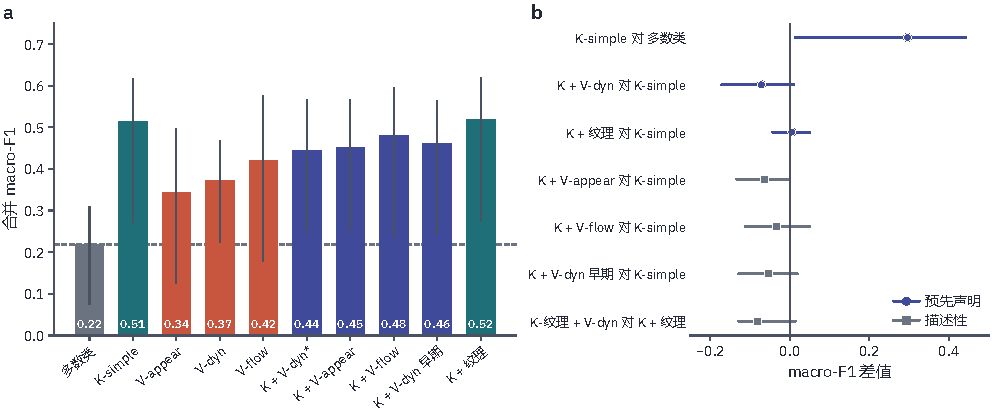
\includegraphics{fig3_results_zh.pdf}
\caption{(a) 多数类、运动学模型（青色）、纯视频模型（红色）和融合模型（蓝色）的合并 macro-F1。误差线为 95\% 用户级 bootstrap 区间；虚线为多数类得分；* 表示预先声明的主多模态模型。(b) macro-F1 的配对差值及其 95\% 用户级 bootstrap 区间。圆点为实验前声明的三个比较，方块为描述性比较。}
\label{fig:results}
\end{figure}

与文献相比，\citet{zia2018rmis} 用近似熵特征在 LOUO 下报告了缝合任务 88.2\% 的准确率。这个数字与我们的结果不能直接比较。在 39 个合并预测下，准确率以 2.56 个百分点为步长变化，88.2\% 不可能出现，所以该文的评估一定使用了不同的试次集合或不同的汇总方式；而且它报告的是准确率而不是 macro-F1。深度网络在 JIGSAWS 上报告的近乎完美的结果大多采用 LOSO，此时测试外科医生也贡献了训练试次\citep{fawaz2018cnn, funke2019video}。我们的 bootstrap 区间在 macro-F1 上宽约 0.25 至 0.4，说明八位外科医生能分辨的差异十分有限\citep{varoquaux2018cv}：只要有一位外科医生的预测类别改变，macro-F1 就可能变化 0.1 以上。

\subsection{成功与失败案例分析}

图~\ref{fig:confusion} 展示了错误出现的位置。三个运动学和多模态模型都能较好地识别新手（K-simple 的 F1 为 \FNMOne{}），对中级的识别中等（F1 \FIMOne{}），但几乎从不识别专家（F1 \FEMOne{}）。在十个专家试次中，K-simple 把五个判为新手、四个判为中级、一个判为专家。图~\ref{fig:users} 按外科医生给出了细分。新手 B、G 和中级 C、F 大多被正确分类（4/5 或 5/5），而专家 D 在每个运动学模型中只有一个试次正确，专家 E 则一个都没有。这种失败有其结构性原因。当一位专家被留出时，训练集中只剩一位专家外科医生，分类器学到的可能是这位外科医生的个人特点，而不是专家的共同之处；身份探针表明这很容易发生：K-simple 仅凭单个试次就能识别外科医生，平衡准确率为 \IdKSimple{}，而随机水平只有 0.125（图~\ref{fig:audit}a）。试次节奏也帮不上忙。专家试次时长的中位数为 \DurE{}\,s，与中级的 \DurI{}\,s 接近，远低于新手的 \DurN{}\,s（图~\ref{fig:data}a），因此时长可以区分新手和受过训练的外科医生，却无法区分两个受训类别。

\begin{figure}[htbp]
\centering
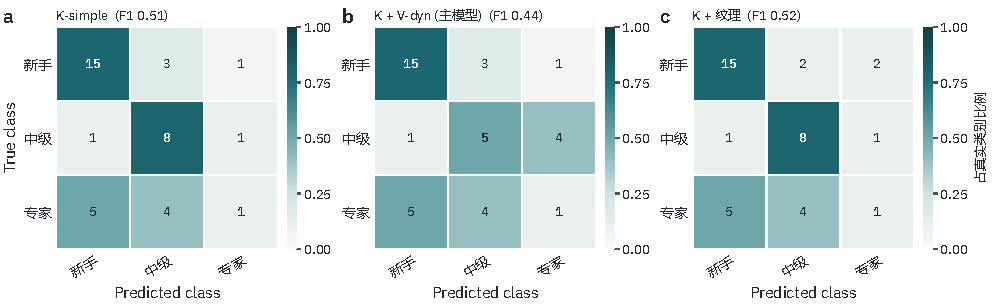
\includegraphics{fig4_confusion_zh.pdf}
\caption{(a) K-simple、(b) 主多模态模型和 (c) 加入运动纹理的 K-simple 的合并混淆矩阵。数字为试次数，颜色表示占真实类别的比例。}
\label{fig:confusion}
\end{figure}

\begin{figure}[htbp]
\centering
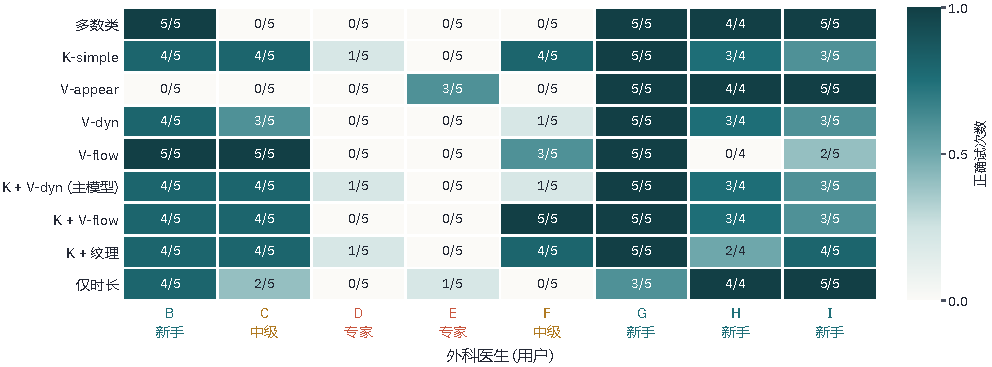
\includegraphics{fig5_users_zh.pdf}
\caption{所选模型在每位被留出外科医生上的正确试次数。每一列是一个 LOUO 折，下方标注该外科医生的技能等级。除 V-appear 外，专家 D 和专家 E 是所有模型的主要失败点；V-appear 则在新手 B 和两位中级外科医生上失败。}
\label{fig:users}
\end{figure}

图~\ref{fig:cases} 在单个试次层面呈现了同样的模式。最明显的成功案例是节奏符合其类别典型水平的试次：新手试次 G001 用时 \CaseGZeroOneDur{}\,s，被判为新手的概率为 \CaseGZeroOnePPred{}；中级试次 C004 用时 \CaseCZeroFourDur{}\,s，被判为中级的概率为 \CaseCZeroFourPPred{}。两位专家则朝相反方向出错，这正是一个学到了“某个人”而不是“某一类”的模型会有的表现。留出 E 时，训练集中唯一的专家是 D，其试次用时 \DurRangeD{}\,s；E 的试次用时 \DurRangeE{}\,s，对专家而言可能显得偏慢，于是五个试次全被判为新手，其中 E001（\CaseEZeroOneDur{}\,s）的新手概率为 \CaseEZeroOnePPred{}，专家概率只有 \CaseEZeroOnePTrue{}。留出 D 时，训练集中唯一的专家是 E，此时训练集里最快的试次属于中级（\DurRangeCF{}\,s），D 的五个试次中有四个被判为中级，包括全数据集最短的试次 D005（\CaseDZeroFiveDur{}\,s），其中级概率为 \CaseDZeroFivePPred{}，专家概率为 \CaseDZeroFivePTrue{}。并非所有错误都能用时长解释。新手 I 的最后两个试次都用时约两分钟，却以很高的置信度被判为中级（I005，\CaseIZeroFiveDur{}\,s，中级概率 \CaseIZeroFivePPred{}），说明模型也会对试次长度以外的 K-simple 特征作出反应。

\begin{figure}[htbp]
\centering
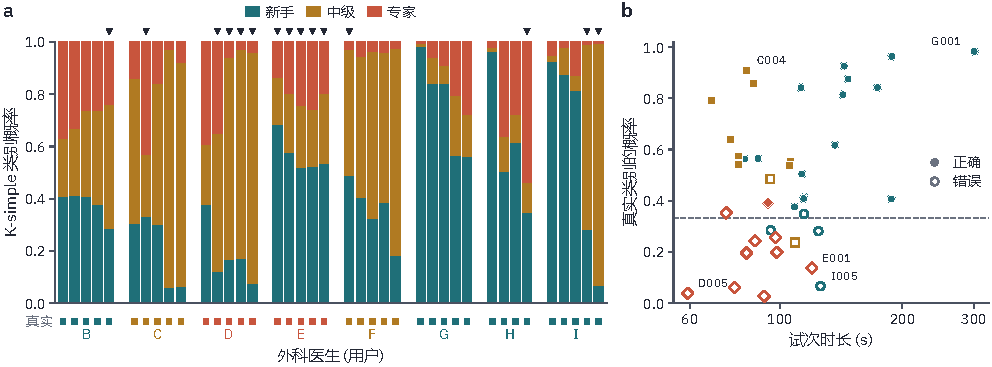
\includegraphics{fig7_cases_zh.pdf}
\caption{K-simple 的试次级预测。(a) 每个试次的类别概率，按被留出的外科医生分组；柱下方块表示真实类别，三角标出预测错误的试次。(b) 真实类别的概率与试次时长（对数坐标）的关系；实心标记为预测正确，空心标记为预测错误，虚线为随机水平（1/3）。图中标注的试次在正文中讨论。}
\label{fig:cases}
\end{figure}

节奏审计显示了运动学信号中有多少是速度。仅用时长的分类器（C1）的 macro-F1 为 \FCOne{}，远高于多数类；K-simple 各特征与 log 时长的绝对相关系数中位数为 \PaceKSimple{}。在训练折内把每个 K-simple 特征对 log 时长做残差化后（C2），macro-F1 从 \FMOne{} 降到 \FCTwo{}；加入纹理特征块时也是如此（C2t，\FCTwoT{}）。因此，K-simple 能迁移到新外科医生的技能信息，主要由试次耗时及随之缩放的量承载（图~\ref{fig:audit}b）。在台式模型任务中，受训外科医生更快，用它区分新手与受训者是合理的，但它并不是质量的度量，这也解释了为什么专家类别被漏判。

\begin{figure}[htbp]
\centering
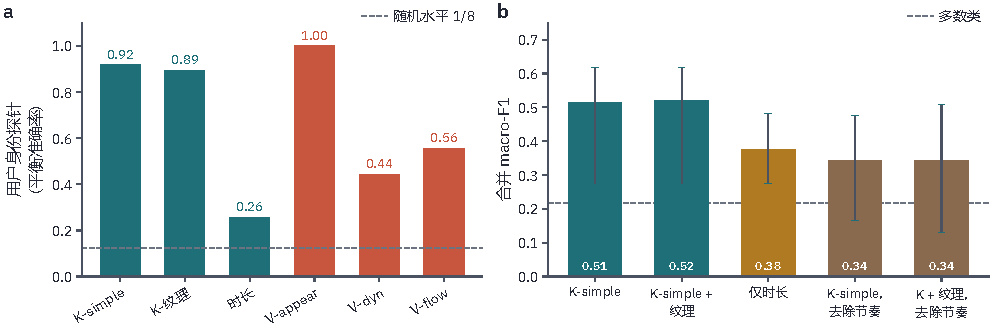
\includegraphics{fig6_audit_zh.pdf}
\caption{捷径审计。(a) 在每个特征块上进行八分类外科医生身份探针的平衡准确率（按试次分层五折），虚线为随机水平。(b) 运动学模型与仅时长分类器、以及在每个训练折内去除与 log 时长线性相关成分后的同一运动学特征的 macro-F1 对比。}
\label{fig:audit}
\end{figure}

视频结果可以用同样两个机制解释。V-appear 能完美识别外科医生（平衡准确率 \IdVAppear{}），但作为技能分类器只有 \FMTwoA{}；图~\ref{fig:users} 呈现出“识别录制场次”的特征模式：新手 G、H、I 的所有试次和专家 E 的三个试次判断正确，而新手 B 和两位中级外科医生的每个试次都判断错误。因此它在专家 E 上的偶然成功不太可能反映技能。V-dyn 的设计目的是抵消静态外观，它携带的身份信息少得多（\IdVDyn{}），却与节奏密切相关：其与 log 时长的绝对相关系数中位数为 \PaceVDyn{}，高于 K-simple。因此它只是提供了运动学模型已有信息的一份更嘈杂的拷贝。在等权重后期融合中，只要视频分类器在运动学判断正确的外科医生上出错，融合结果就会变差。最明显的例子是中级外科医生 F：K-simple 在 5 个试次中对 4 个，V-dyn 只对 1 个，平均之后融合模型只对 \UFMThree{}（图~\ref{fig:users}）。V-flow 在 F 上与运动学互补（融合后 \UFMThreeC{}），但在新手 H 上完全失败，因此其融合结果仍低于单独的运动学模型。

运动纹理改进失败的原因可以从特征本身看出。每个器械的对数无量纲加加速度与 log 时长的相关系数达到 $|r| = \PaceKTextureMax{}$，这与已知的无量纲加加速度对动作时长敏感的结论一致\citep{hogan2009smoothness}；纹理特征块识别外科医生的能力也几乎与 K-simple 相当（\IdKTexture{}）。因此这十个纹理特征在很大程度上重复了 K-simple 已经包含的节奏和身份信息。此外，我们的特征块远小于 \citet{zia2018rmis} 使用的特征集，后者在每个运动学通道上都计算了近似熵；我们没有测试更大的特征集，因为它不在预先声明的协议中，看过这些结果后再去选择它会使比较产生偏差。

\subsection{实现与配置细节}

内层 LOUO 选择在大多数折中选出了较强的正则化（K-simple 在八折中有七折的 $C$ 介于 0.01 与 0.1 之间），这与训练外科医生数量少的情况相符。对 V-appear，内层循环在八折中有六折选择了四个主成分。按照协议，外层折 C、D、E、F 各跳过了一个内层折。K-simple 按外科医生平均的逐折准确率为 \FoldAccMOne{} $\pm$ \FoldSdMOne{}（均值 $\pm$ 标准差），正是这种逐折离散度使我们报告带用户级区间的合并指标，而不是各折的平均值。代码按阶段组织为若干模块（\texttt{data.py}、\texttt{features\_kin.py}、\texttt{features\_video.py}、\texttt{evaluate.py}），\texttt{run\_all.py} 可在约五分钟内从原始数据复现所有模型、预测文件和统计量；\texttt{make\_tables.py} 和 \texttt{make\_figures.py} 可在不重新训练的情况下，从保存的结果重新生成本报告的表格和图。

\section{结论与讨论}

\subsection{主要发现}

我们在官方留一用户协议下，把 JIGSAWS 缝合任务的试次分为新手、中级或专家，遵循本课题规定的实验，并在第一个结果出来之前用书面协议固定了所有模型和比较。简单的试次级运动学统计量明显优于多数类（macro-F1 \FMOne{} 对 \FMZero{}，精确置换 $p = \PMOne{}$）。来自采样帧的视频特征单独使用时没有超过随机水平，无论后期还是早期融合，把它们与运动学结合都没有超过单独的运动学模型；预先声明的主融合模型得分为 \FMThree{}。针对性改进，即参照背景文献思路设计的运动纹理特征，使 macro-F1 基本不变（\FMFour{}）。捷径审计解释了这一模式的大部分。运动学统计量中可迁移的信号主要是试次节奏，它能区分新手与受训外科医生，却不能区分中级与专家；而专家只有两位，模型无法学到两人的共同之处，因此专家类几乎从未被识别出来。整帧外观特征能完美识别外科医生，却不携带可迁移的技能信号；场景动态特征则主要重复了节奏信息。

主要的设计选择取决于问题的规模。只有八位外科医生、每个受训类别只有两位，因此我们使用带强正则化和嵌套选择的线性模型以及冻结的预训练特征，而没有训练深度网络；由于每折只含一个类别时逐折 macro-F1 没有定义，我们报告合并 macro-F1、用户级 bootstrap 区间和精确的用户级置换检验。这些选择让结果如实反映其不确定性，代价是区间较宽，无法分辨小于约 0.1 至 0.2 的 macro-F1 差异。

\subsection{优点与不足}

本研究的主要优点是结论不依赖于看过结果之后做出的选择。折划分是官方的，被留出的外科医生从不参与任何拟合，每个模型只评估一次，负面结果与正面结果一并报告。审计还揭示了分类器实际使用的是哪些信息，这对此类系统的任何临床应用都很重要。第~\ref{sec:differences}~节列出了本方法与背景文献和相关工作的四点不同；对本研究的结论而言，最重要的是以外科医生为单位处理不确定性，以及直接测量身份和节奏捷径。

本方法也有明显的不足。它最擅长的是节奏能揭示的东西，即在标准化台式任务上区分新手和受训外科医生；一旦受训外科医生之间的差别在于质量而非速度，它就很可能失效，专家类的结果正说明了这一点。模型只在七位外科医生上训练，一位不典型的外科医生就可能主导一折；自报技能标签衡量的是练习时长，而不是实际表现。视频特征描述的是整帧画面，没有关注针、线或组织，而观察者恰恰是在这些地方看到运动学无法捕捉的质量差异。最后，等权重后期融合是一种粗糙的组合规则，会让较弱的模态拖累较强的模态。

\subsection{未来方向}

最有效的一步是增加外科医生数量，例如在留出外科医生后用 JIGSAWS 的全部三个任务训练，或加入其他数据集，因为仅凭一位训练外科医生无法学到专家类。区分中级与专家可能需要与节奏关联更弱的特征，例如手势级的时间与错误事件，或按时长归一化的动作质量；本文引入的身份探针和节奏对照可以用来检验任何这类特征。在视频方面，在器械尖端附近区域或缝合最终状态上计算的特征，可能捕捉到组织处理和成品质量，而运动学和我们的整帧描述符都观察不到这些。在训练折内选择融合权重，或采用倾向于较强模态的融合规则，也能避免这里观察到的稀释效应。任何此类扩展都应保持严格的 LOUO 协议和书面预注册，因为外科医生数量少，事后选择很容易过拟合。

\subsection*{AI 工具使用声明}

我们使用了 Claude Code 及 Anthropic 的两个模型 Claude Fable 5.1 和 Claude Opus 5.5，用于规划实验、编写与调试代码、运行实验、生成图表，以及起草和修改本报告与演示文稿。本组审阅了代码、结果和文字，并对所提交工作的内容和质量负责。


\small
\bibliographystyle{unsrtnat}
\bibliography{../report/references}

\end{document}
